\section{Iluminación}
Para la iluminación de la escena he utilizado una combinación de 3 luces, como se pedía en el guion, y de un cambio del color de fondo para que las zonas que no son iluminadas sean visibles.

\bigskip

Voy a dividir en subsecciones las explicaciones del color de fondo y de la iluminación:

\subsection{Color de fondo}

% rescribir
El color de fondo por defecto que tienen las escenas es el negro, haciendo que cuando se utiliza iluminación, las zonas no iluminadas por los puntos de luz aparezcan negros por completo. Para solucionar esto es necesario modificar el color de fondo por un gris oscuro, para que se pueda ver toda la escena.

\bigskip

Para ello, es necesario irse a los menús de arriba y darle clic a ``Rendering'' $\rightarrow$ ``Environment''.

\begin{figure}[H]
    \centering
    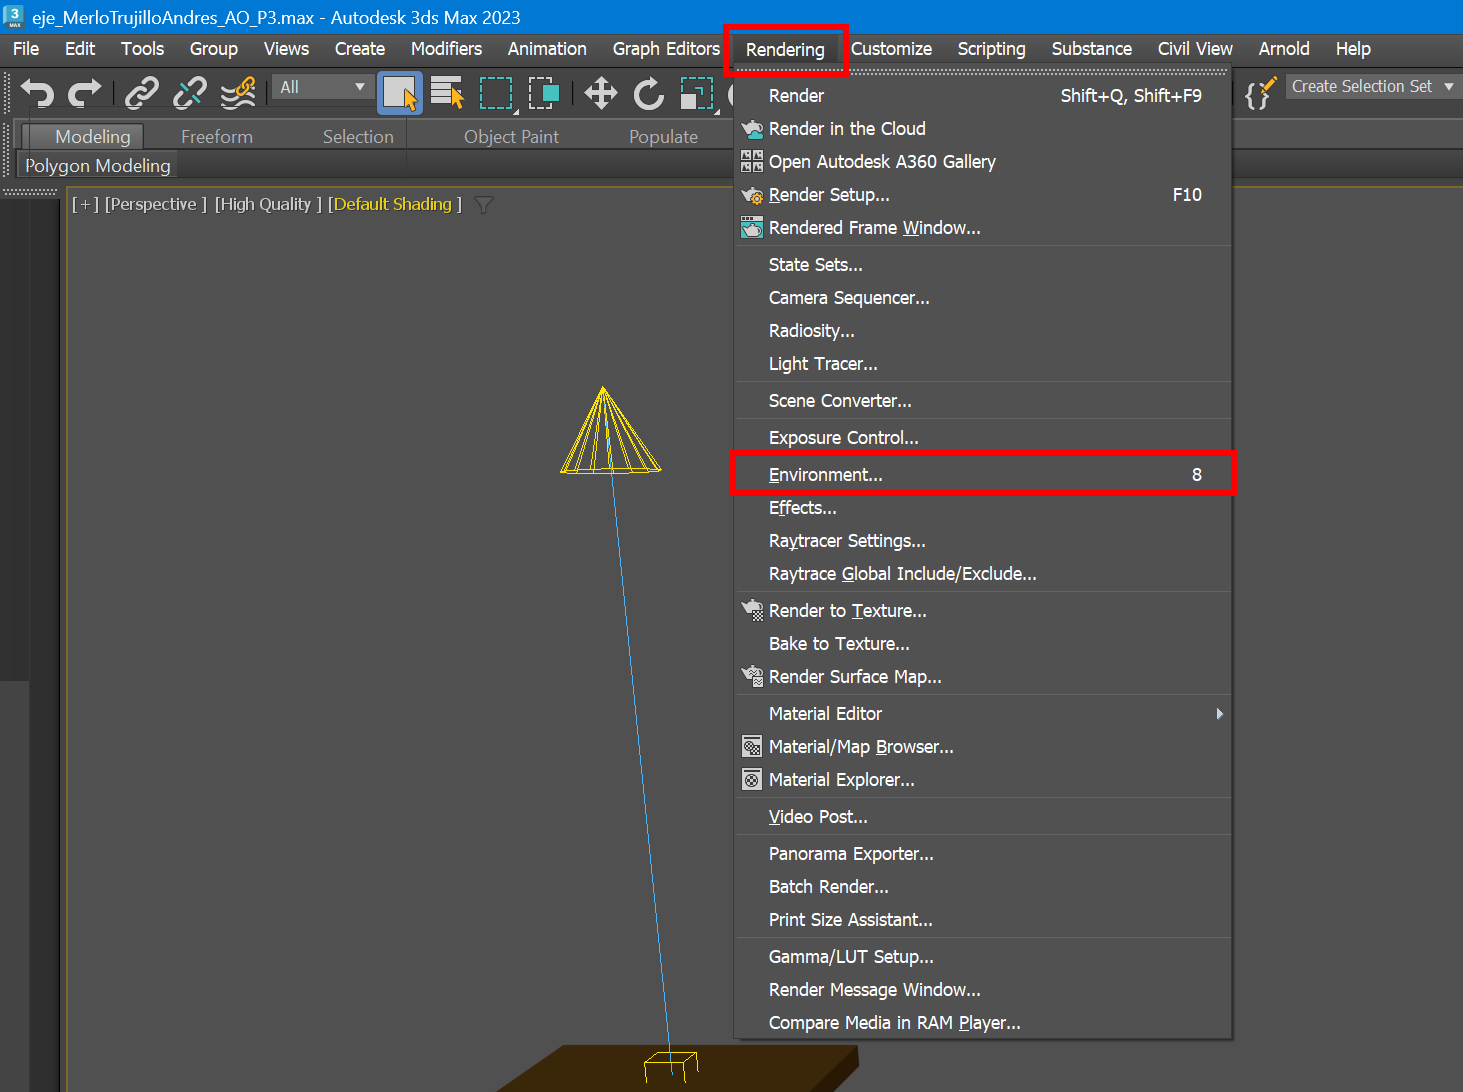
\includegraphics[width=0.7\textwidth]{imagenes/misc/bg-color1.png}
    \caption{Ubicación de la opción para cambiar el color de fondo.}
 \end{figure}

Se abrirá una ventana a la que hay que darle al rectángulo de selección de color de la sección ``Background'' y elegir un tono más claro.

\begin{figure}[H]
    \centering
    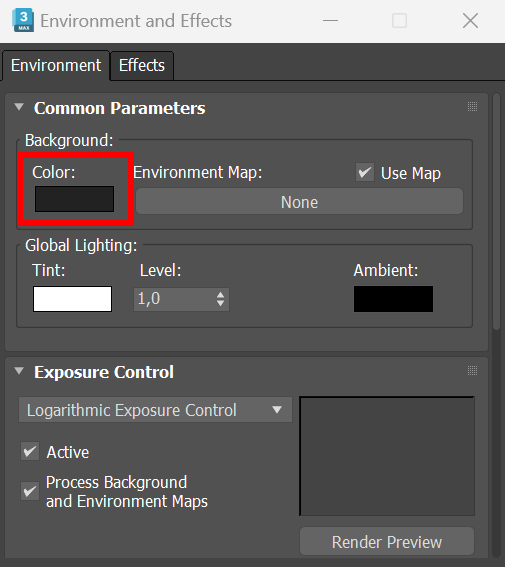
\includegraphics[width=0.5\textwidth]{imagenes/misc/bg-color2.png}
    \caption{Ventana con la opción para cambiar el color de fondo.}
 \end{figure}

\subsection{Puntos de luz de la escena}
Para la iluminación de la escena he utilizado 3 \textit{Target Lights} junto a una distribución de luz de tipo \textit{Spotlight}, permitiéndome modificar el cono de luz para que solo ilumine las bases, para el caso de las luces de los extremos, y el trampolín, para el caso de la luz intermedia.

\bigskip

Esta subsección la voy a dividir a su vez en distintas subsecciones, una para cada luz puesta en la escena.

\subsubsection{Luz de la izquierda}
% rescribir

Los \textit{keyframes} para el foco de la izquierda son:

\begin{itemize}
    \item \textbf{Instante 0: }La luz ahora mismo se encuentra encendida y de color blanco. Se hace para que la animación inversa funcione correctamente.
    \item \textbf{Instante 38: }La luz se encuentra exactamente igual que en el instante anterior.
    \item \textbf{Instante 58: }La luz pasa a tener color rojo y apagarse (intensidad a 0) porque la pelota ha saltado de la plataforma.
    \item \textbf{Instante 150: }Exactamente igual que en el instante anterior. Se realiza para hacer que la animación inversa funcione bien y porque la pelota no está en la base.
\end{itemize}

\newpage

Las curvas de animación son las siguientes:

\begin{figure}[H]
    \centering
    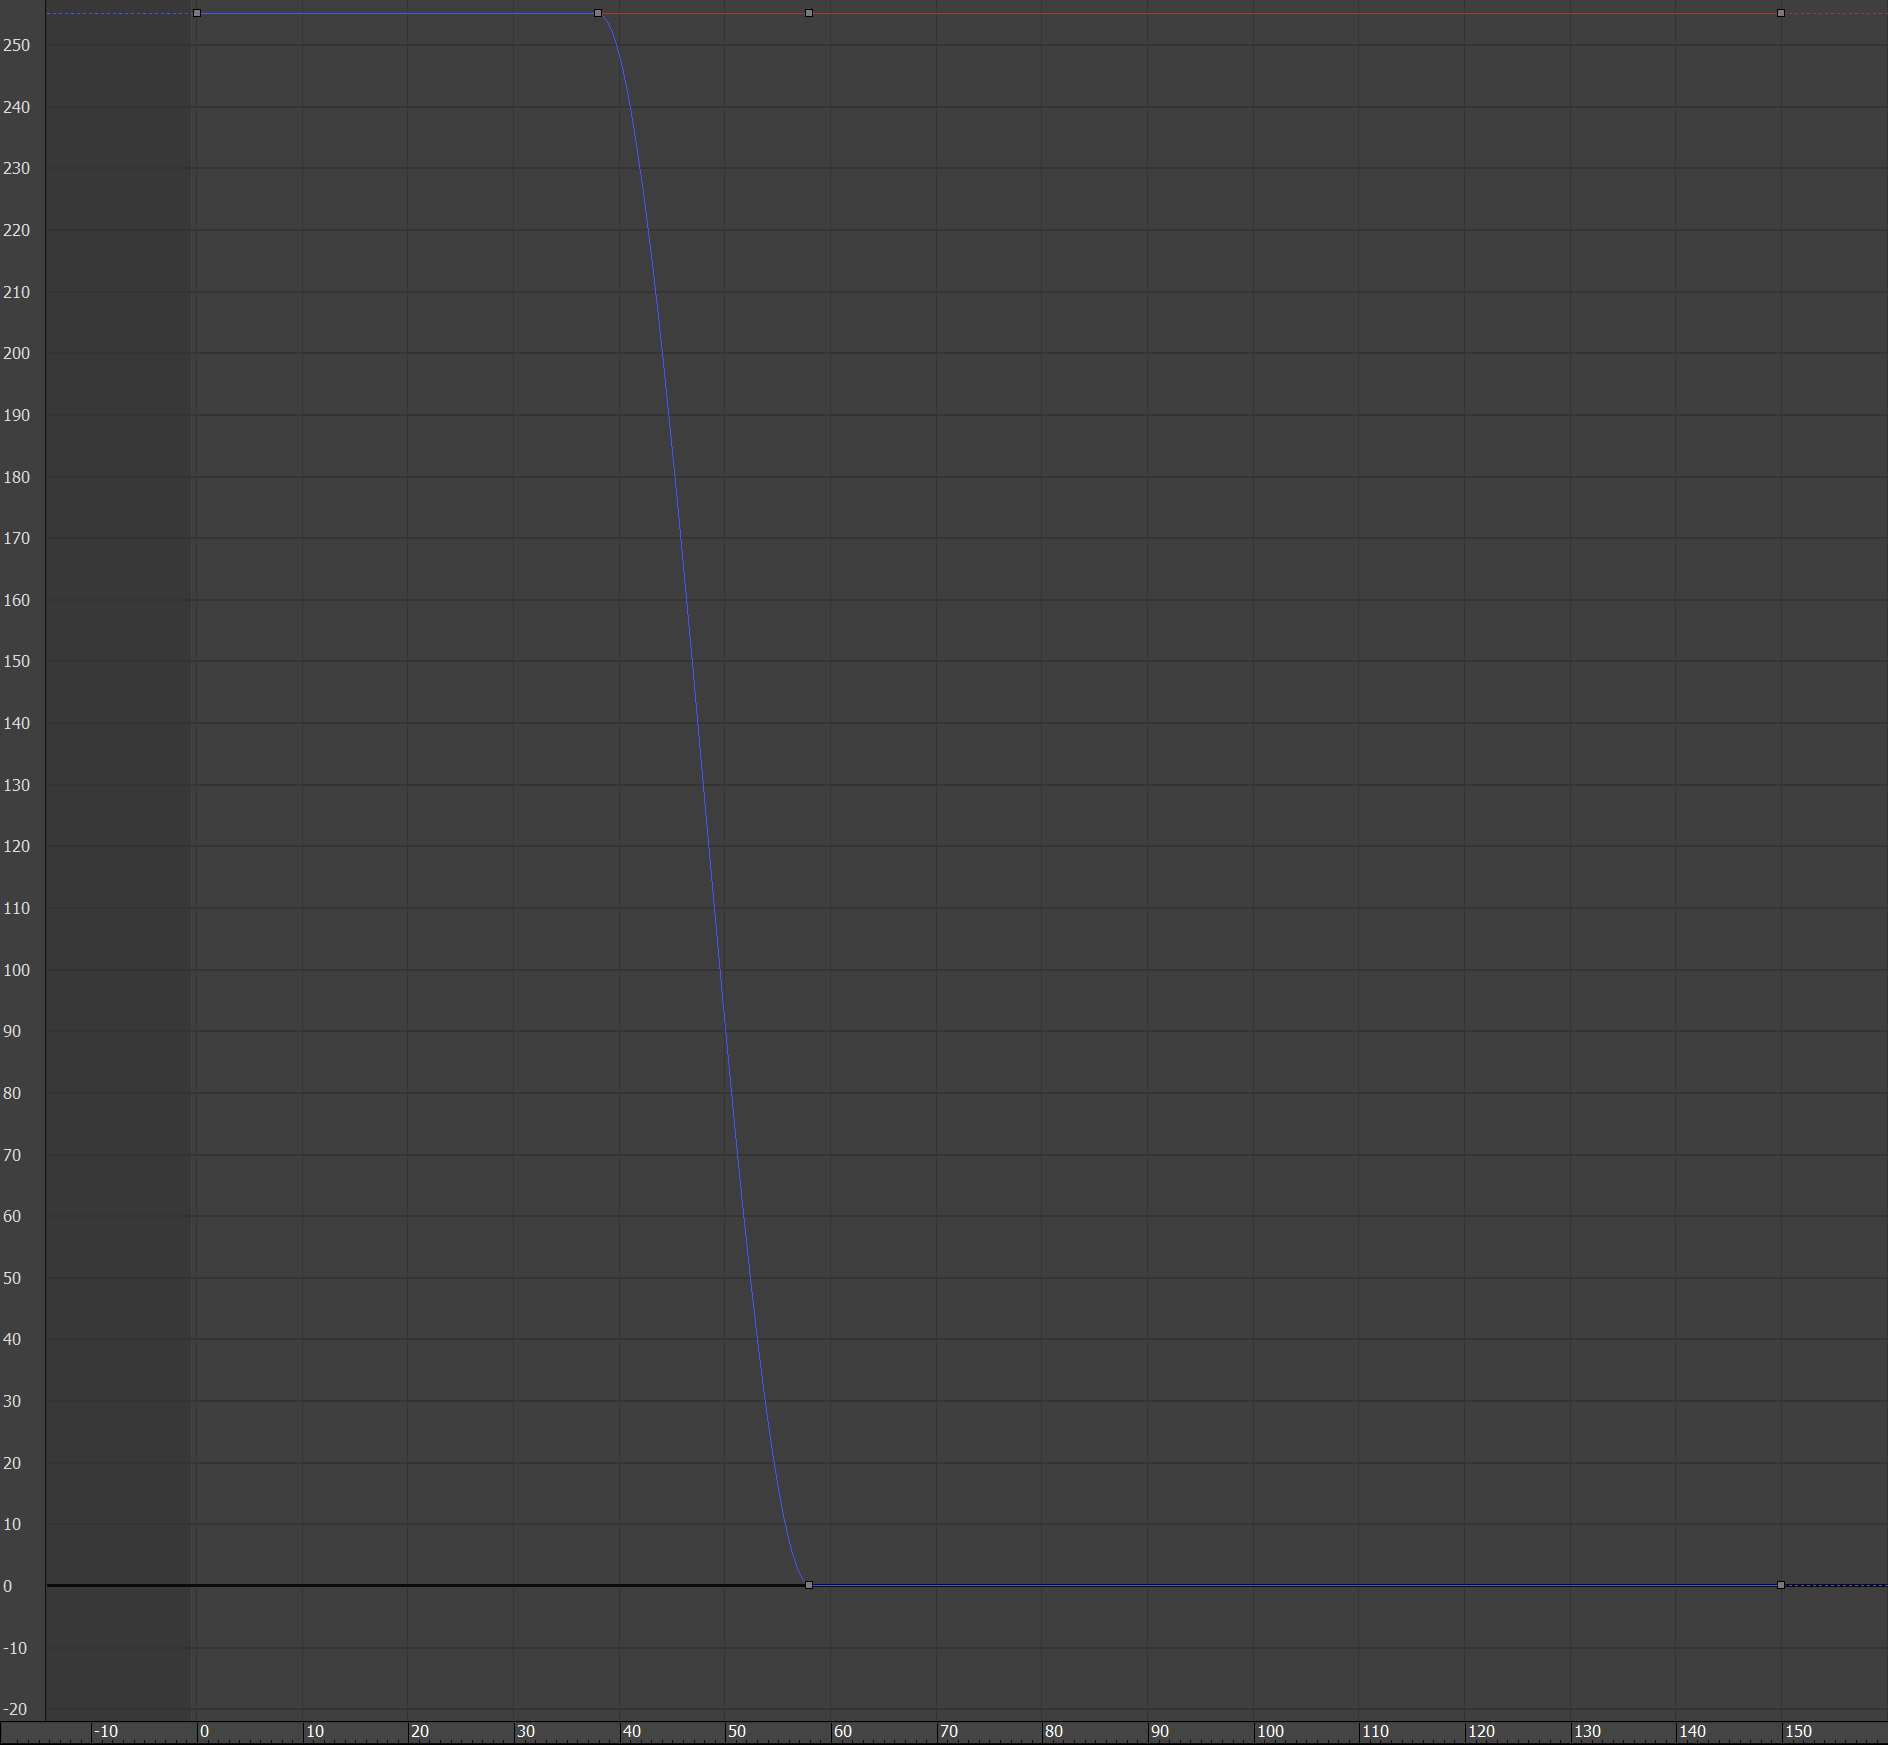
\includegraphics[width=0.6\textwidth]{imagenes/curvas/LL/filter.png}
    \caption{Curva que representa el color de la luz con respecto al tiempo.}
 \end{figure}

En la curva he usado una función \textit{Slow-in/Slow-out} para simular la iluminación progresiva que tendría una luz incandescente al ser encendidas y apagada.

 \begin{figure}[H]
    \centering
    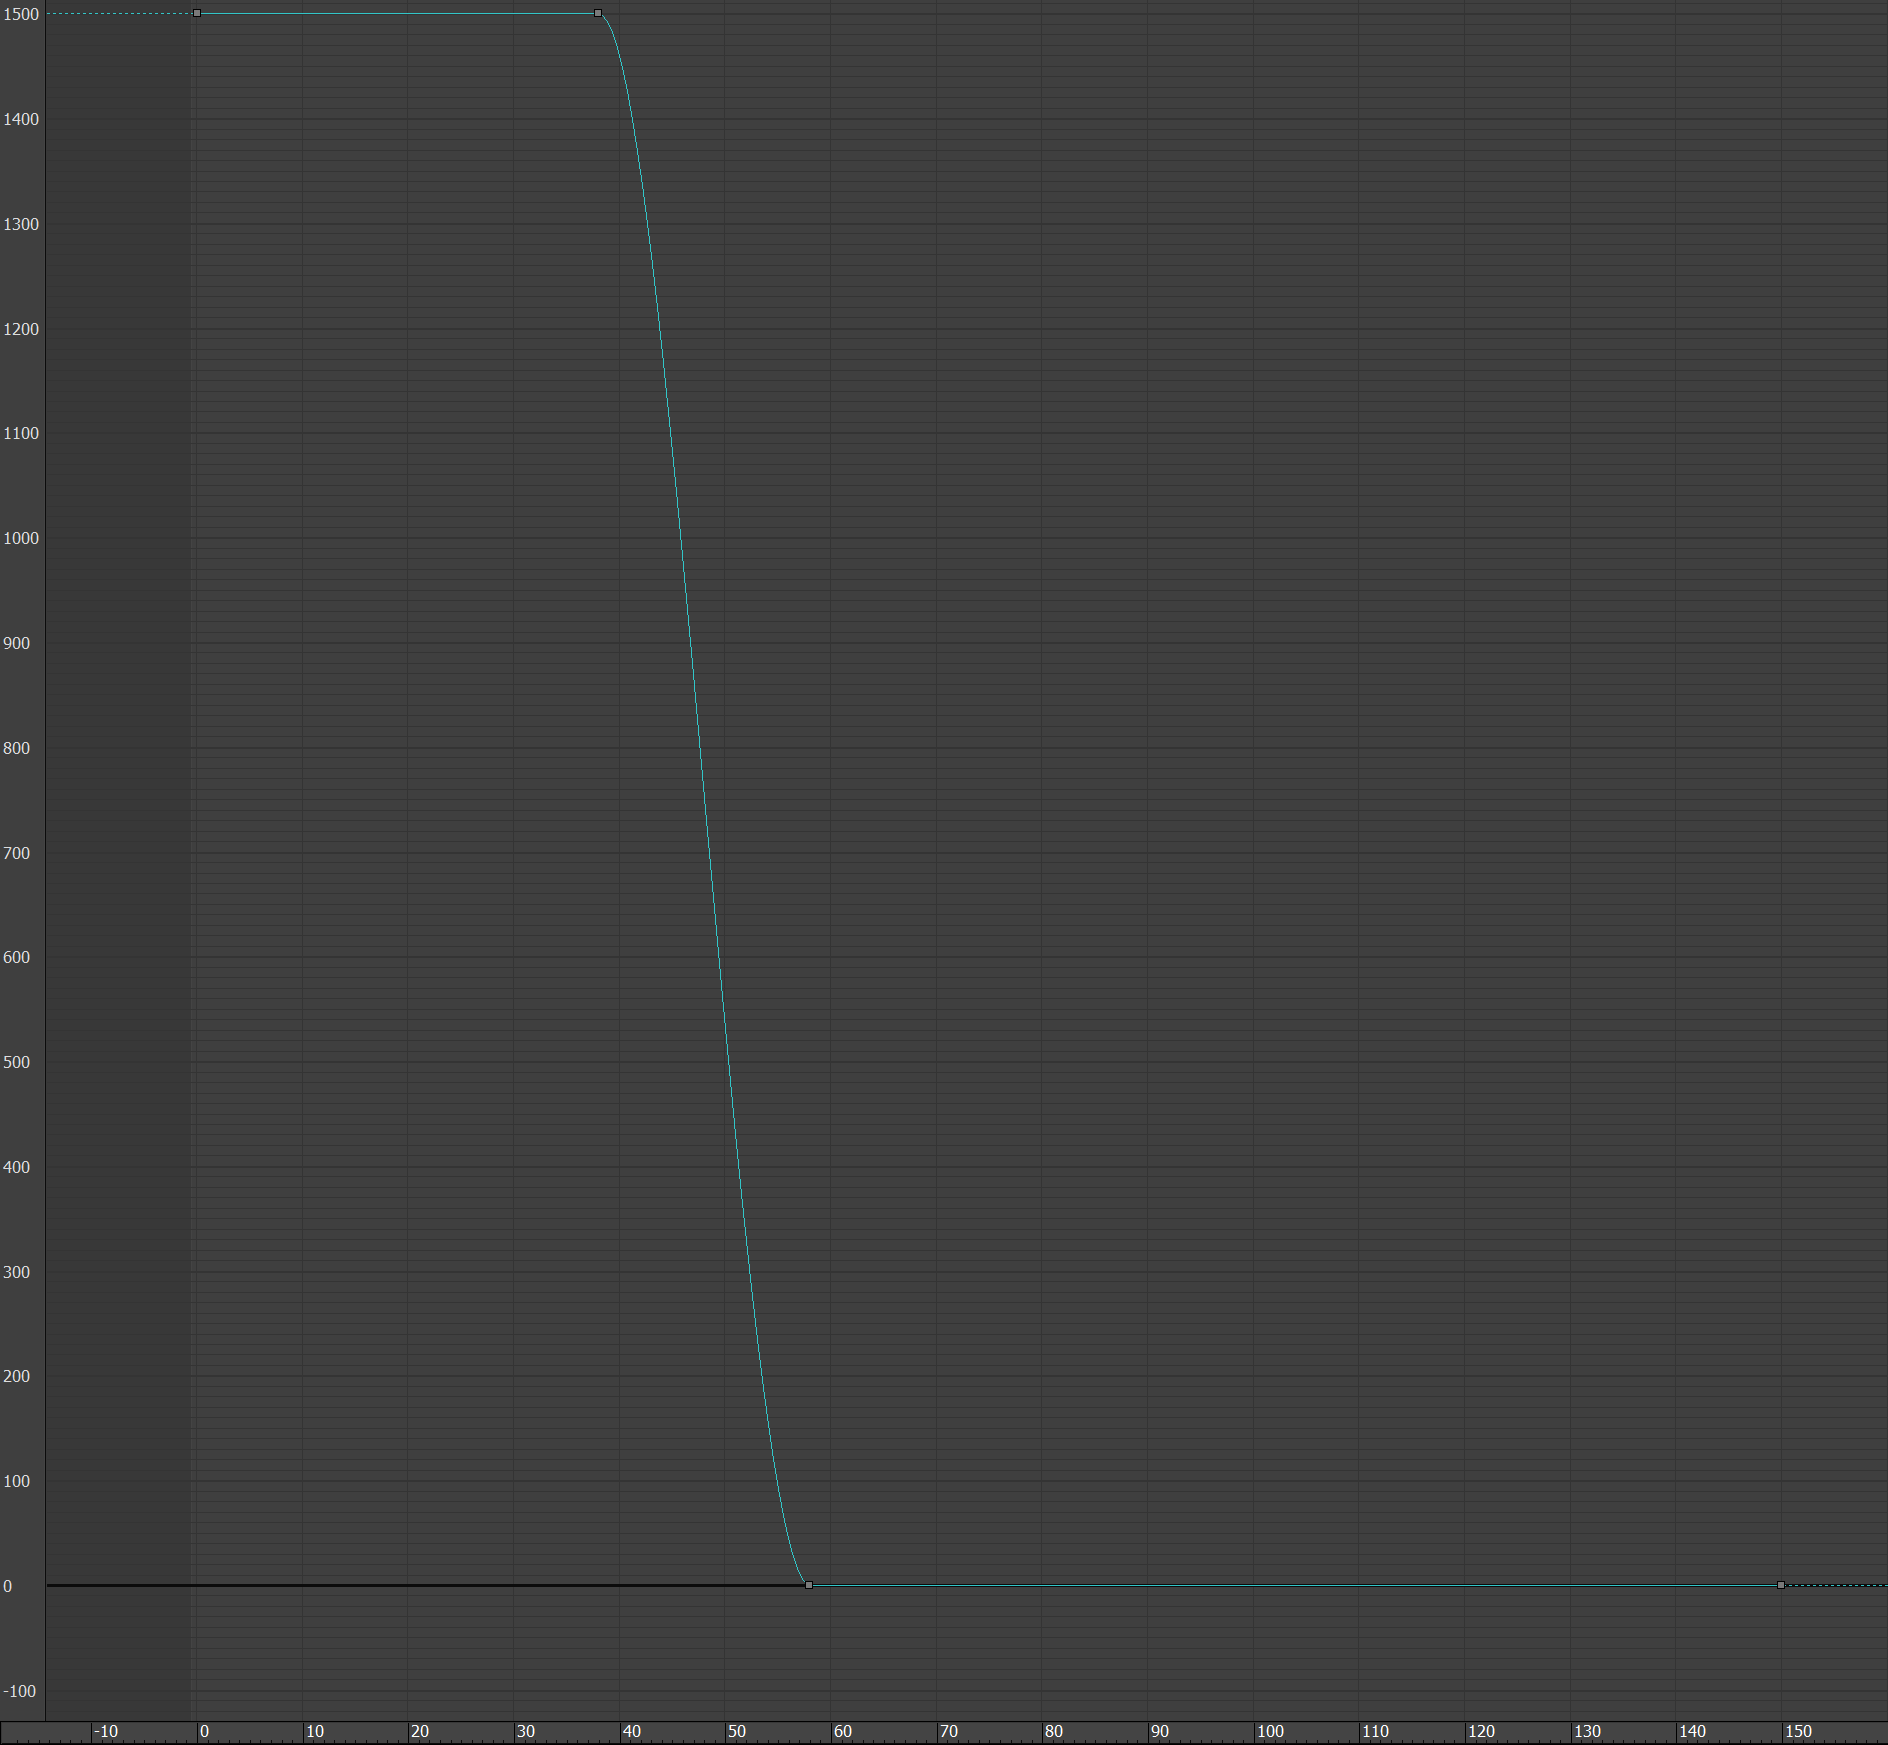
\includegraphics[width=0.6\textwidth]{imagenes/curvas/LL/intensity.png}
    \caption{Curva que representa la intensidad de la luz con respecto al tiempo.}
 \end{figure}

 En esta curva también he usado el mismo tipo de función que en la anterior, con el objetivo de simular el encendido y apagado progresivo que tienen algunas luces, entre ellas las incandescentes como antes.

 \subsubsection{Luz de la derecha}

 El punto de luz del otro extremo que ilumina la otra pelota tiene los mismos \textit{keyframes}, pero comenzando desde el final:

 \begin{itemize}
    \item \textbf{Instante 0: }Se encuentra de color rojo y con la intensidad a 0. Esto se hace para que la animación inversa funcione de manera correcta con las demás componentes y porque no se encuentra la pelota en la base.
    \item \textbf{Instante 92: }La luz sigue exactamente igual que en el instante anterior.
    \item \textbf{Instante 112: }La luz ahora se encuentra iluminada al máximo y de color blanco.
    \item \textbf{Instante 150: }Se encuentra exactamente igual que en el instante anterior, con el objetivo de que la animación inversa funcione correctamente y porque la pelota está rebotando en la base.
 \end{itemize}
 
 \bigskip

Las curvas de animación son las siguientes:

\begin{figure}[H]
    \centering
    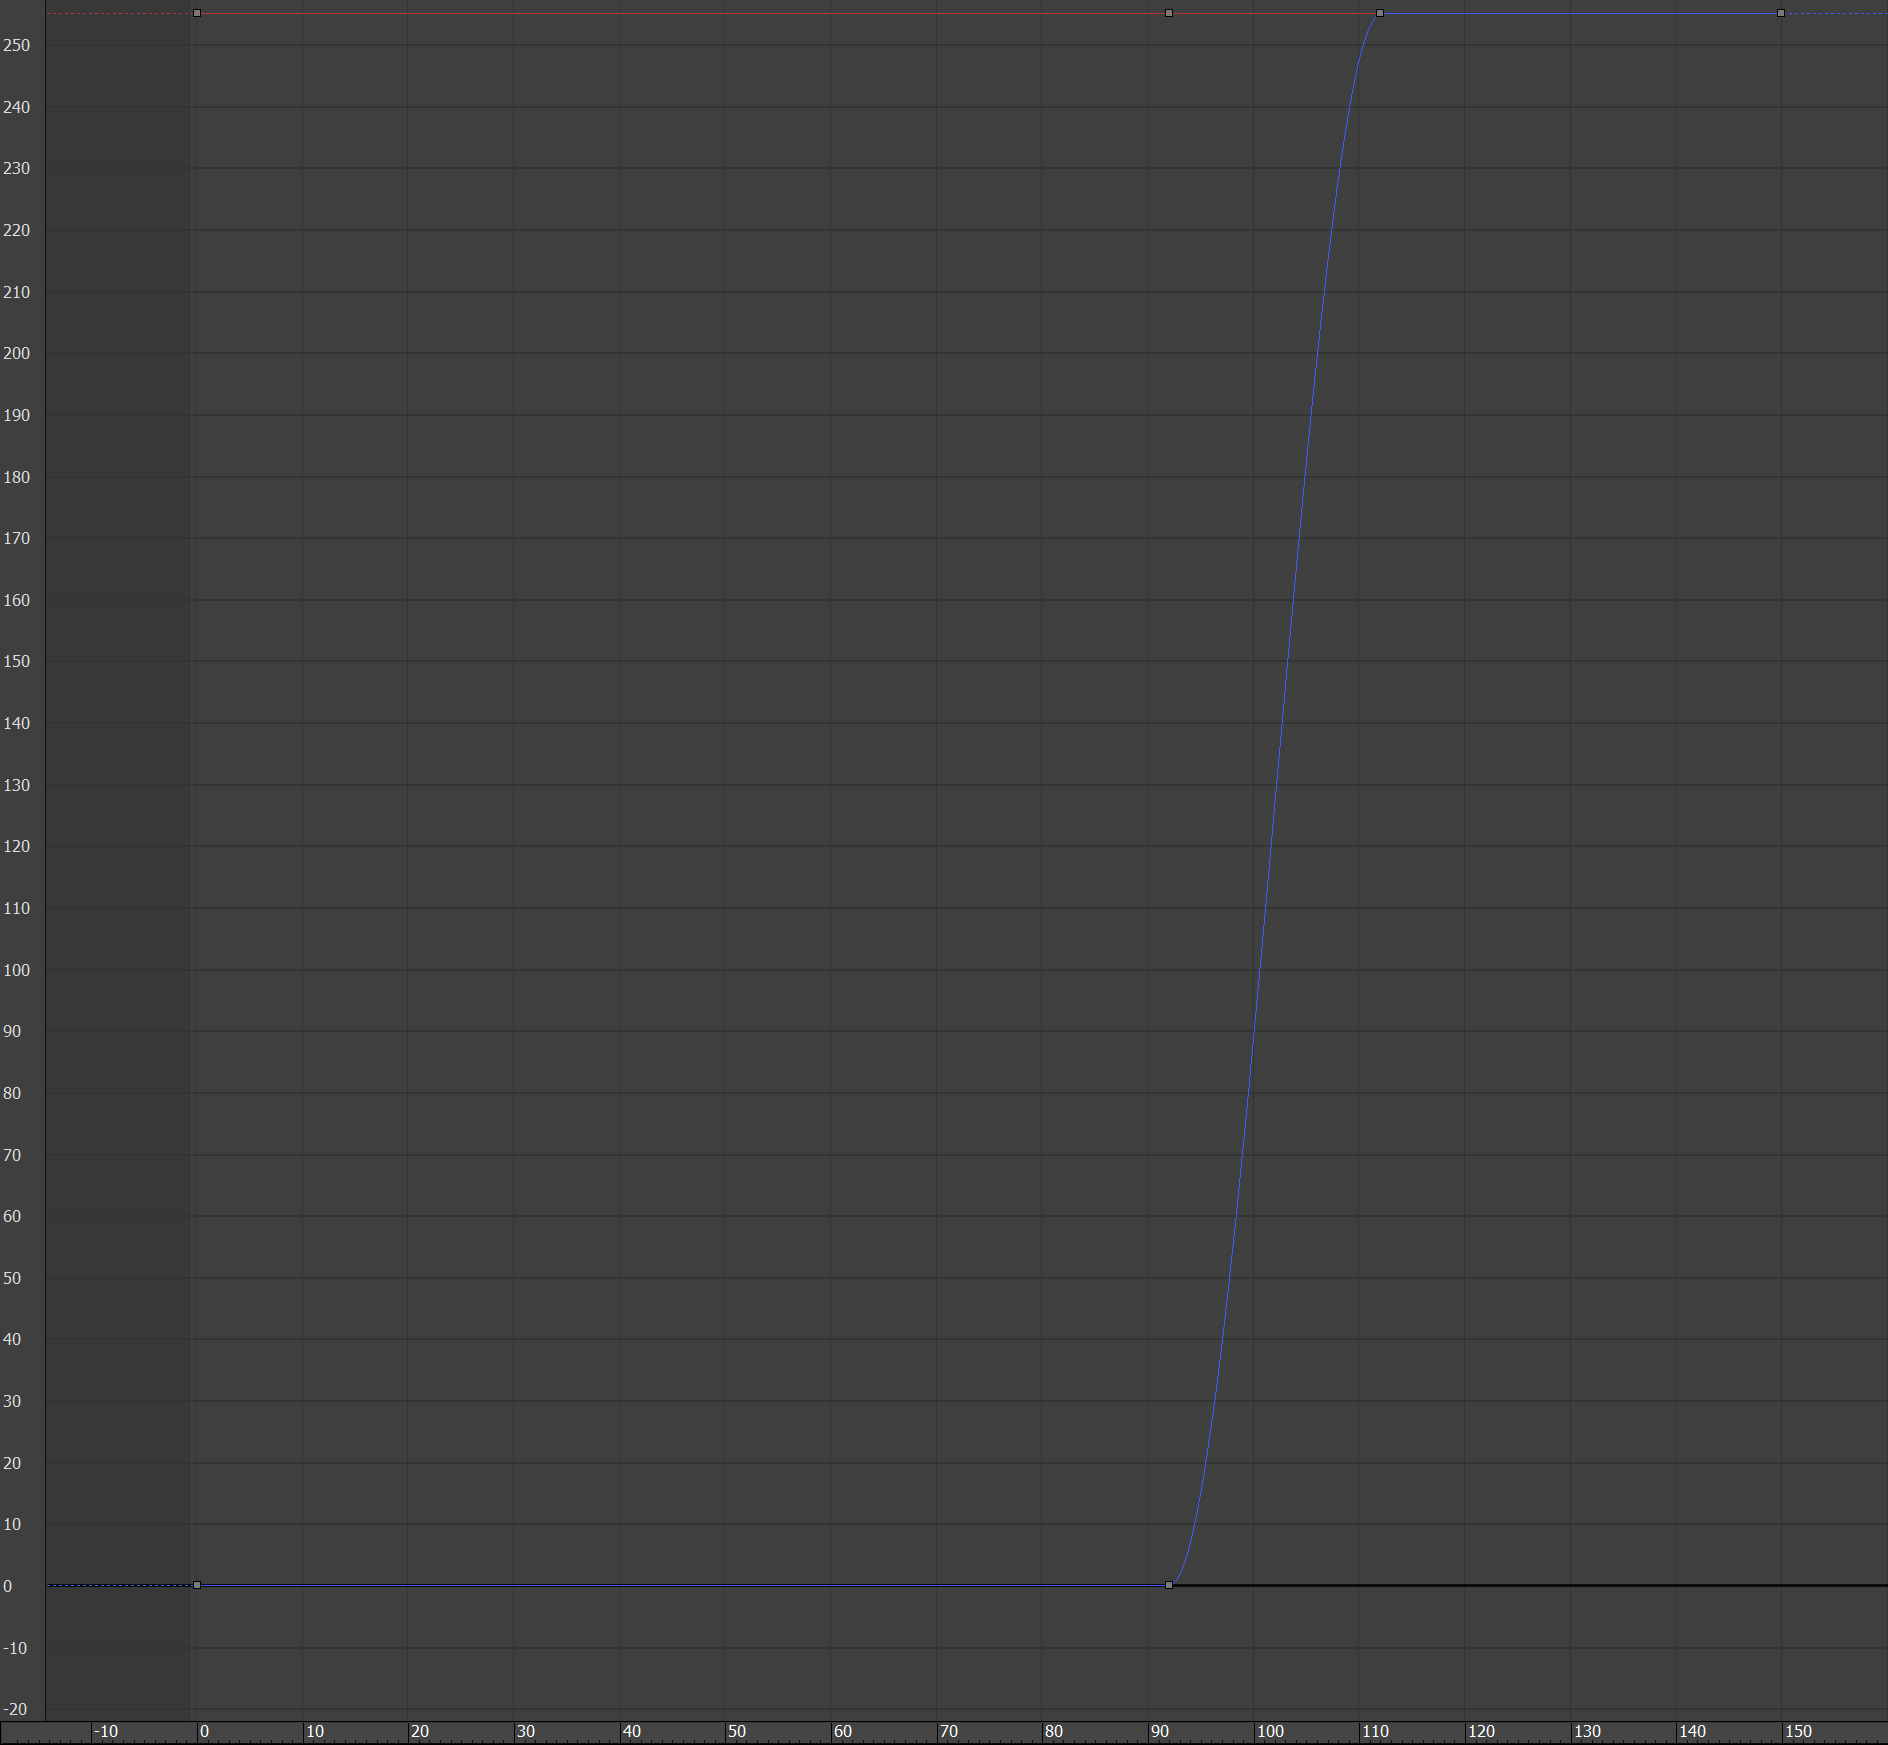
\includegraphics[width=0.6\textwidth]{imagenes/curvas/LR/filter.png}
    \caption{Curva que representa el color de la luz con respecto al tiempo.}
 \end{figure}

 \begin{figure}[H]
    \centering
    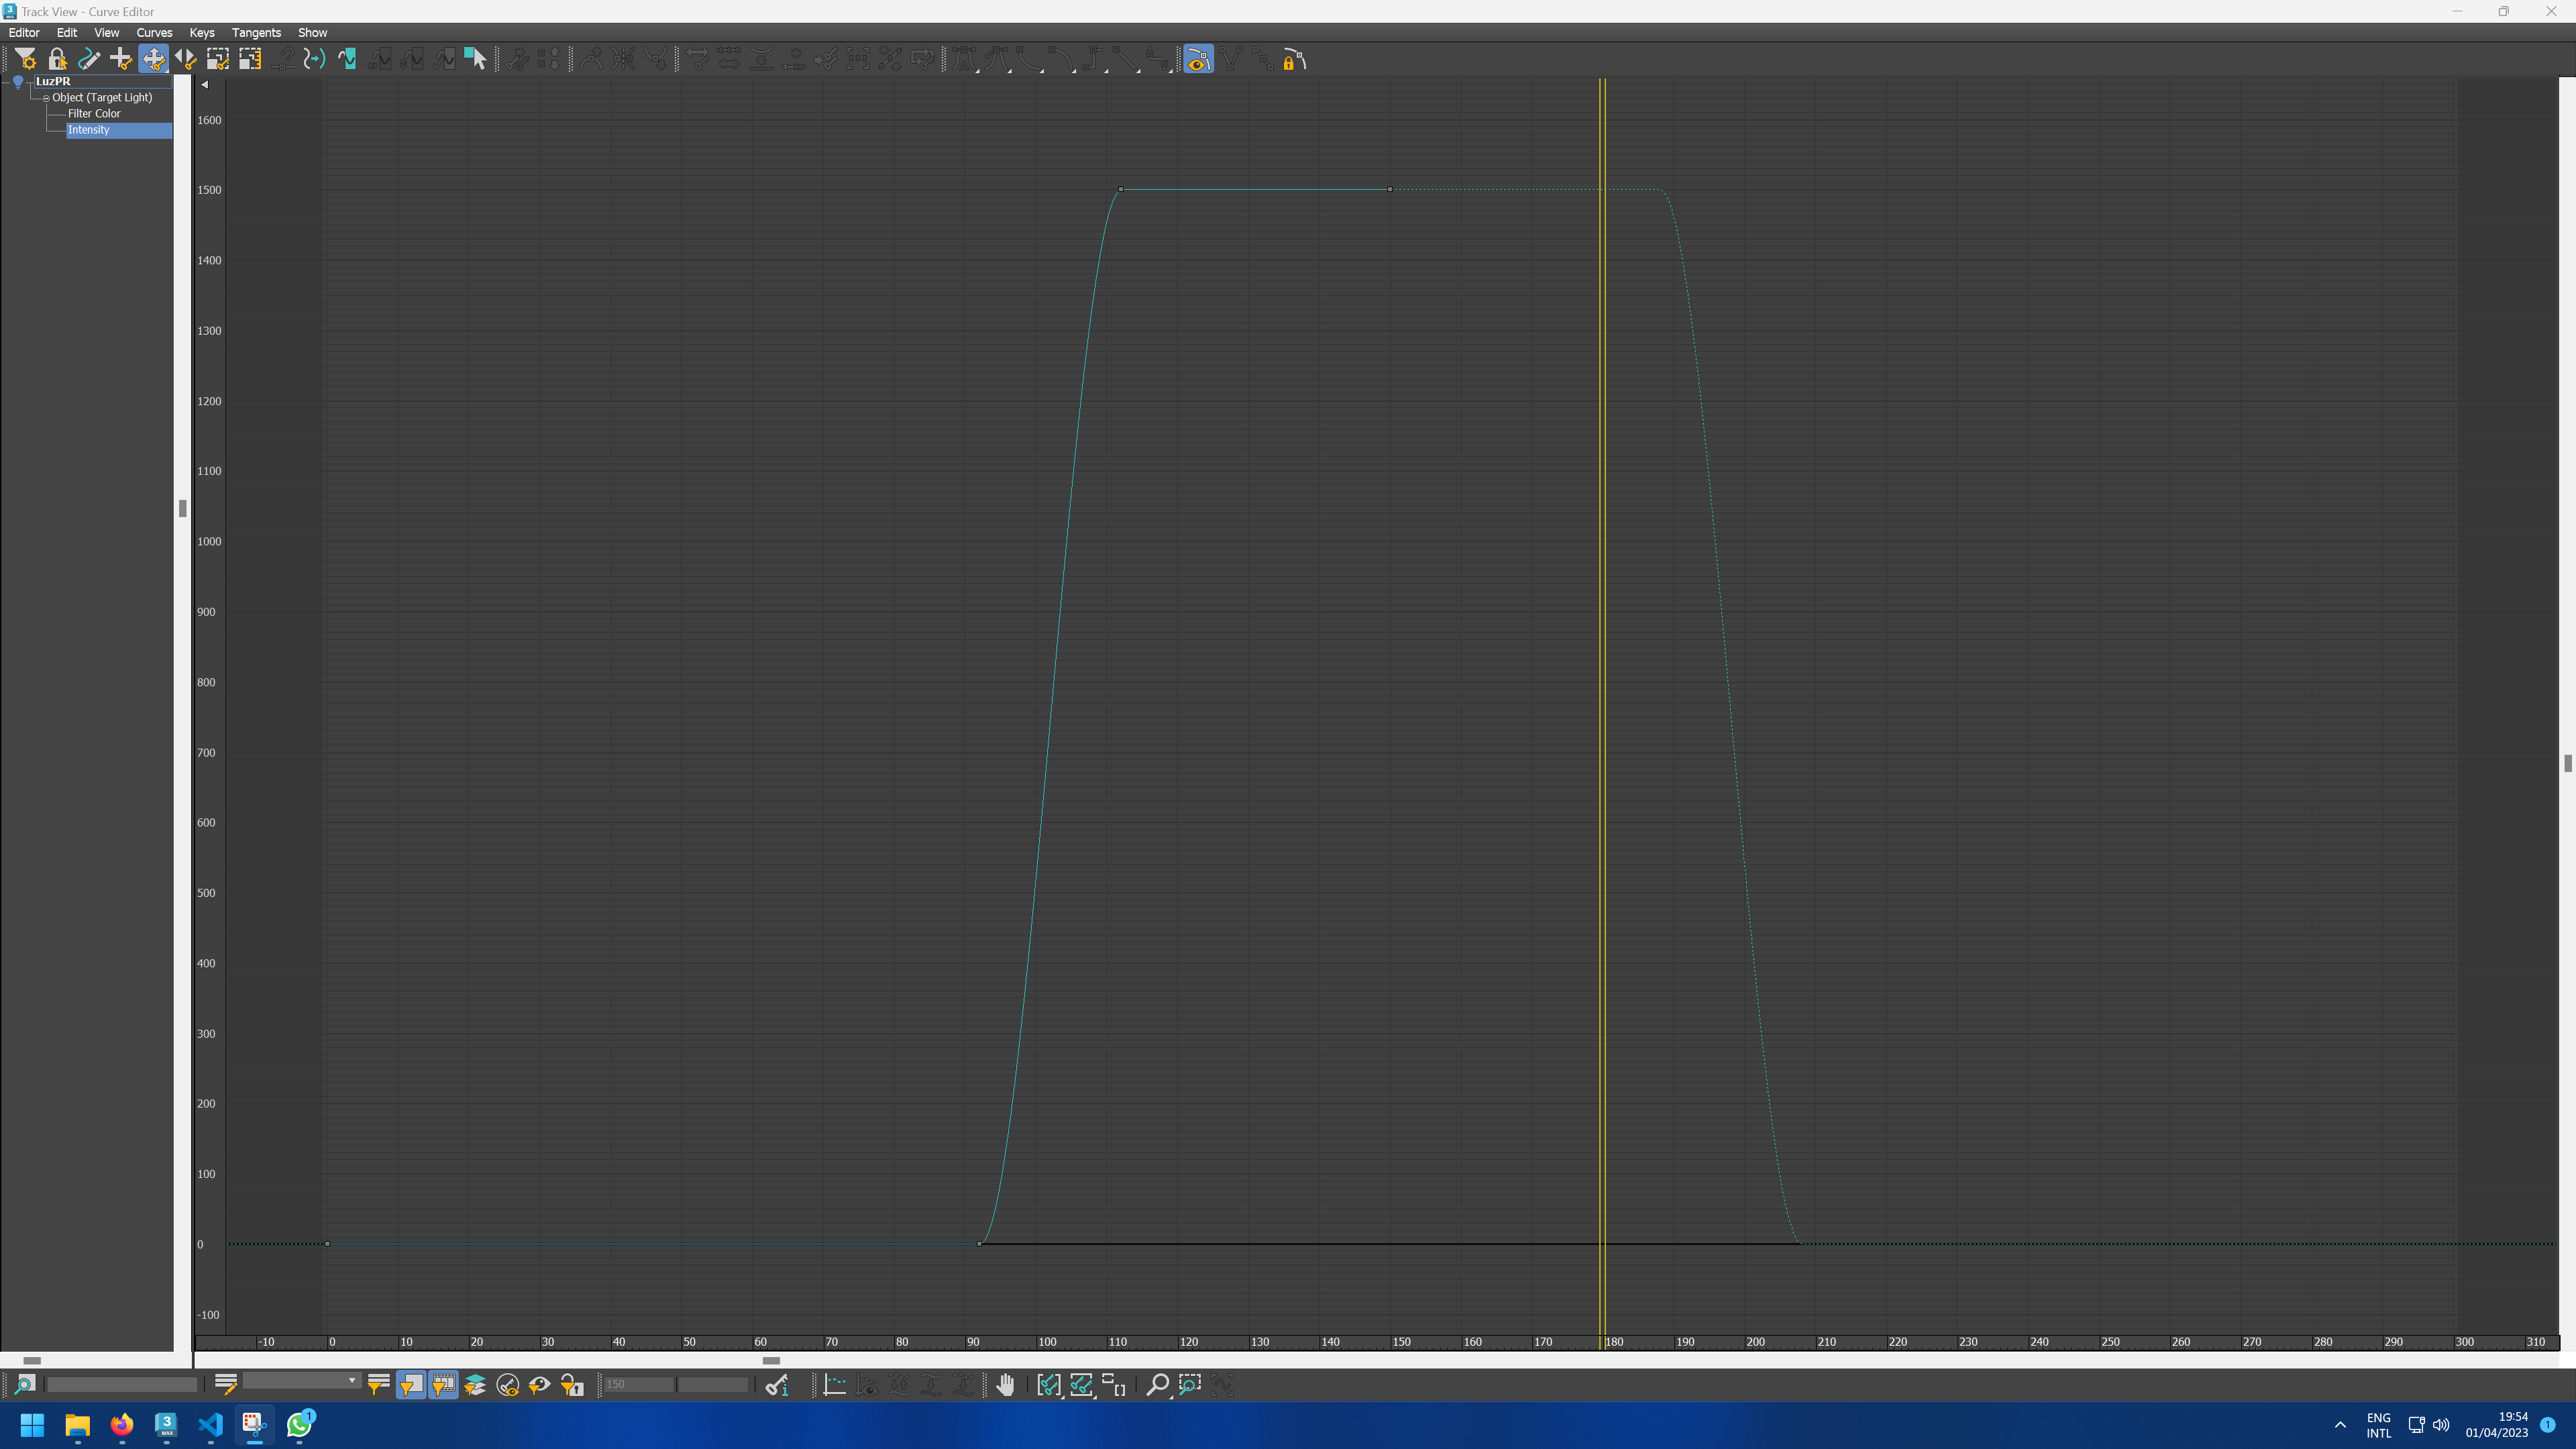
\includegraphics[width=0.6\textwidth]{imagenes/curvas/LR/intensity.png}
    \caption{Curva que representa la intensidad de la luz con respecto al tiempo.}
 \end{figure}

Al igual que con la luz del otro extremo, esta se encenderá y apagará progresivamente, simulando una luz incandescente.


\subsubsection{Luz central}

La luz intermedia, utilizada para iluminar el trampolín, tiene los siguientes \textit{keyframes}:

\begin{itemize}
    \item \textbf{Instante 0: }La luz se encuentra apagada y de color rojo, para hacer la animación inversa correctamente y porque no hay movimiento en el trampolín.
    \item \textbf{Instante 38: }La luz sigue exactamente igual que en el instante anterior.
    \item \textbf{Instante 58: }La luz se encuentra encendida y de color blanco, indicando que hay movimiento en el trampolín.
    \item \textbf{Instante 92: }La luz sigue exactamente igual que antes, ya que todavía hay movimiento en el trampolín.
    \item \textbf{Instante 112: }La luz ahora se encuentra apagada y de color rojo, al no haber más movimiento en el trampolín.
    \item \textbf{Instante 150: }Sigue sin haber movimiento, por lo que sigue apagada y de color rojo. También es para que la animación inversa funcione.
\end{itemize}

\newpage

Y las curvas de animación son:

\begin{figure}[H]
    \centering
    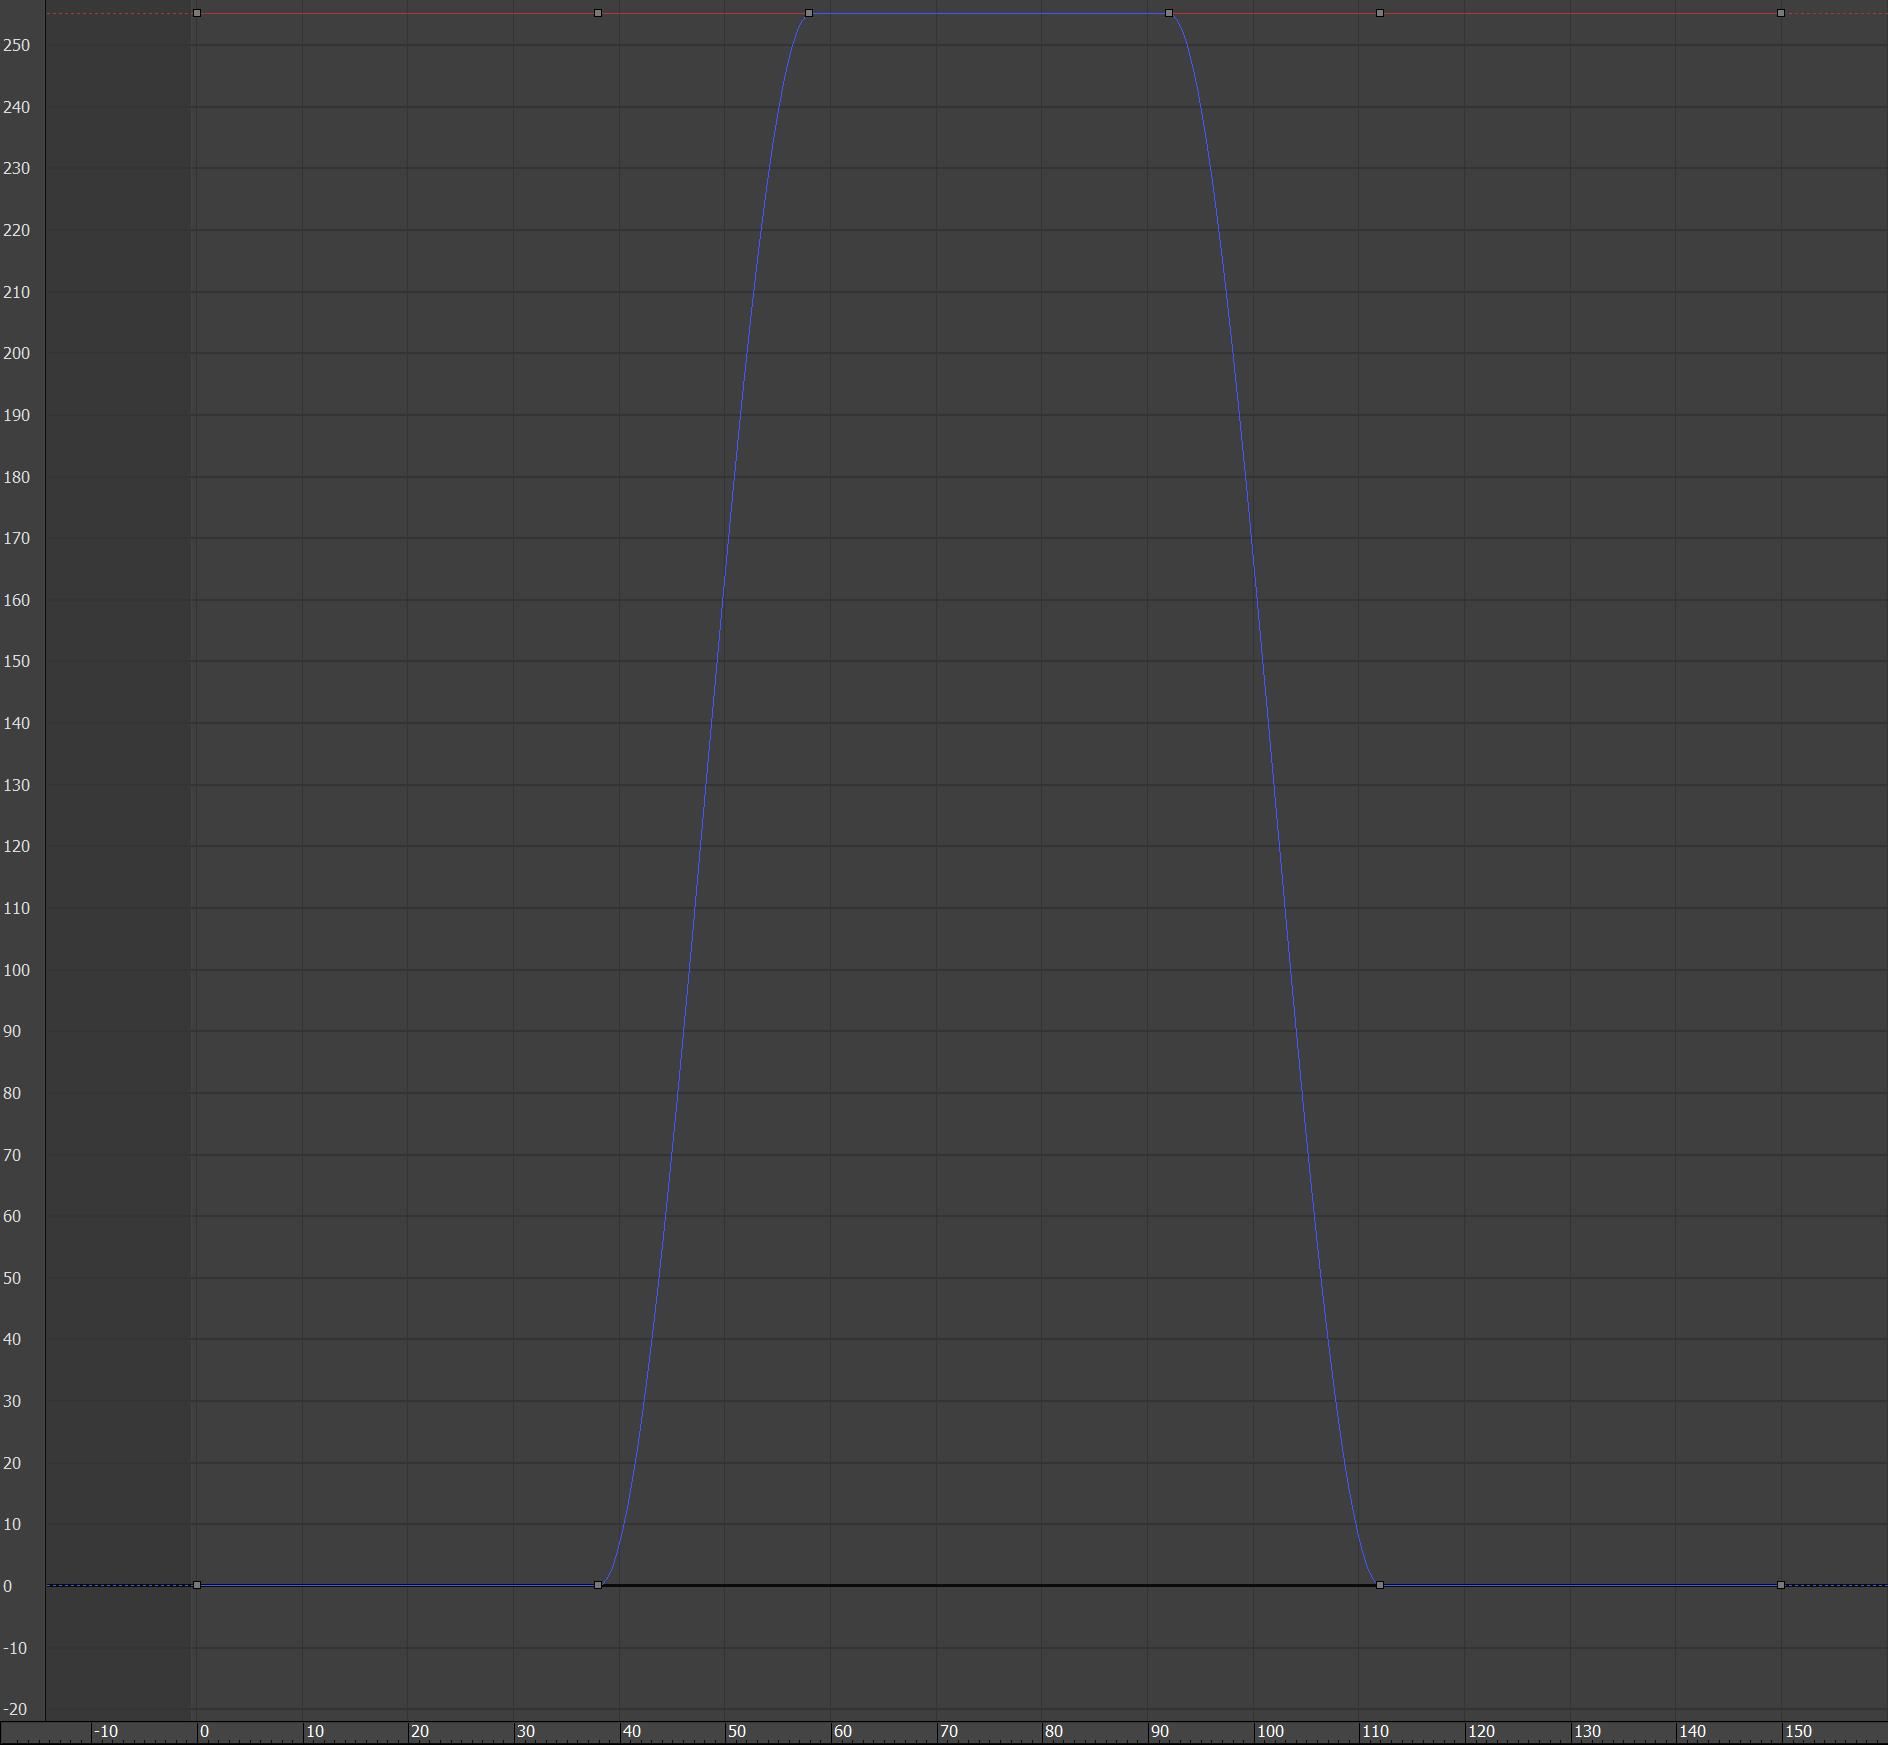
\includegraphics[width=0.6\textwidth]{imagenes/curvas/LC/filter.png}
    \caption{Curva que representa el color de la luz con respecto al tiempo.}
 \end{figure}

 \begin{figure}[H]
    \centering
    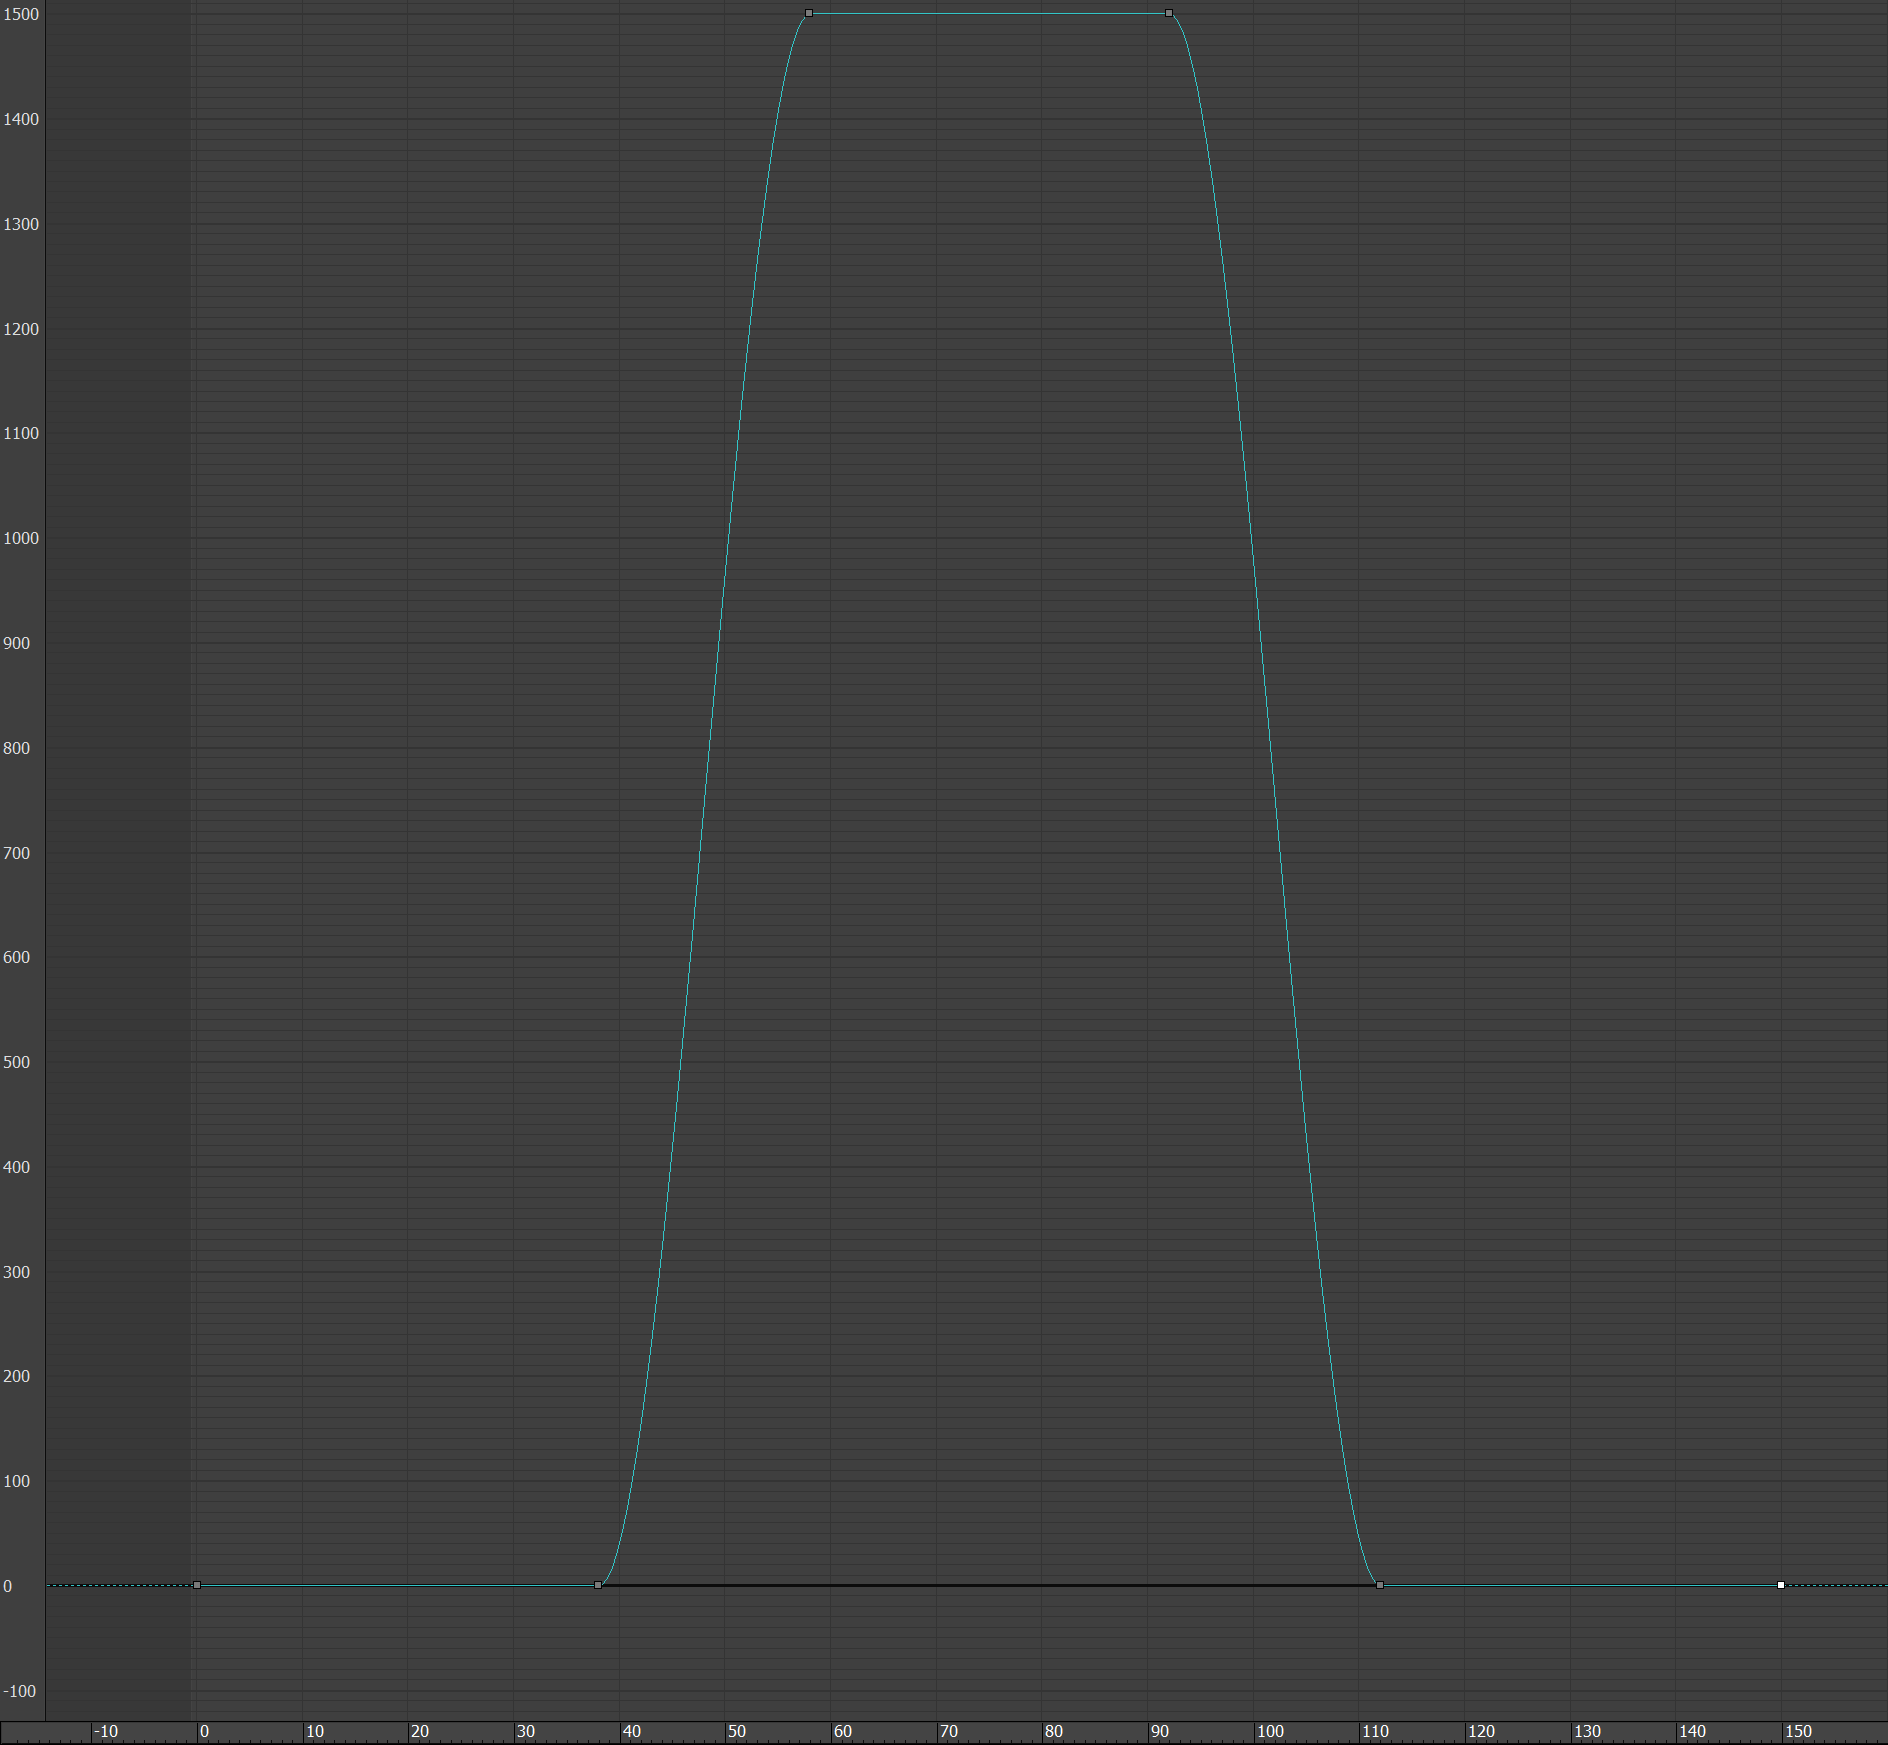
\includegraphics[width=0.6\textwidth]{imagenes/curvas/LC/intensity.png}
    \caption{Curva que representa la intensidad de la luz con respecto al tiempo.}
 \end{figure}

Al igual que con las otras luces, he utilizado una curva \textit{Slow-in/Slow-out} para simular el encendido y apagado progresivo de la luz.